\documentclass{article}
\usepackage[T1]{fontenc}
\usepackage{lmodern}
\usepackage{graphicx}
\usepackage{amsmath,amssymb}
\usepackage[a4paper,margin=2cm]{geometry}
\usepackage[absolute,overlay]{textpos}
\setlength{\TPHorizModule}{1mm}
\setlength{\TPVertModule}{1mm}
\usepackage[indonesian]{babel}
\usepackage{hyperref}
\setlength{\emergencystretch}{2em}
% unit: Halaman 42

\begin{document}

% === Halaman 42 (python/native) ===

42

Diagram Blok RC4:

• Kunci rahasia (secret key) memiliki panjang maksimal 256 karakter (1 karakter = 1byte). 

Jika  panjang kunci kurang dari 256 byte maka karakter-karakter kunci diulang secara 

periodik.

• RC4 menghasilkan luaran berupa kunci-alir (keystream) dengan panjang tak terbatas

Plaintext

Secret Key

RC4



Ciphertext

Keystream

% deskripsi: gambar native xref 188
\noindent
\includegraphics[width=0.85\textwidth]{../../images/python/page_042_img_01.png}

% deskripsi: gambar native xref 190
\noindent
\includegraphics[width=0.85\textwidth]{../../images/python/page_042_img_02.png}

% deskripsi: gambar native xref 192
\noindent
\includegraphics[width=0.85\textwidth]{../../images/python/page_042_img_03.png}

% deskripsi: gambar native xref 194
\noindent
\includegraphics[width=0.85\textwidth]{../../images/python/page_042_img_04.png}

% deskripsi: gambar native xref 196
\noindent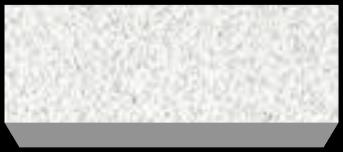
\includegraphics[width=0.85\textwidth]{../../images/python/page_042_img_05.jpeg}

\end{document}
